% Options for packages loaded elsewhere
\PassOptionsToPackage{unicode}{hyperref}
\PassOptionsToPackage{hyphens}{url}
%
\documentclass[
]{article}
\usepackage{amsmath,amssymb}
\usepackage{lmodern}
\usepackage{iftex}
\ifPDFTeX
  \usepackage[T1]{fontenc}
  \usepackage[utf8]{inputenc}
  \usepackage{textcomp} % provide euro and other symbols
\else % if luatex or xetex
  \usepackage{unicode-math}
  \defaultfontfeatures{Scale=MatchLowercase}
  \defaultfontfeatures[\rmfamily]{Ligatures=TeX,Scale=1}
\fi
% Use upquote if available, for straight quotes in verbatim environments
\IfFileExists{upquote.sty}{\usepackage{upquote}}{}
\IfFileExists{microtype.sty}{% use microtype if available
  \usepackage[]{microtype}
  \UseMicrotypeSet[protrusion]{basicmath} % disable protrusion for tt fonts
}{}
\makeatletter
\@ifundefined{KOMAClassName}{% if non-KOMA class
  \IfFileExists{parskip.sty}{%
    \usepackage{parskip}
  }{% else
    \setlength{\parindent}{0pt}
    \setlength{\parskip}{6pt plus 2pt minus 1pt}}
}{% if KOMA class
  \KOMAoptions{parskip=half}}
\makeatother
\usepackage{xcolor}
\usepackage[includeheadfoot,left=0.75in,right=0.75in,top=0.5in,bottom=1.2in]{geometry}
\usepackage{graphicx}
\makeatletter
\def\maxwidth{\ifdim\Gin@nat@width>\linewidth\linewidth\else\Gin@nat@width\fi}
\def\maxheight{\ifdim\Gin@nat@height>\textheight\textheight\else\Gin@nat@height\fi}
\makeatother
% Scale images if necessary, so that they will not overflow the page
% margins by default, and it is still possible to overwrite the defaults
% using explicit options in \includegraphics[width, height, ...]{}
\setkeys{Gin}{width=\maxwidth,height=\maxheight,keepaspectratio}
% Set default figure placement to htbp
\makeatletter
\def\fps@figure{htbp}
\makeatother
\setlength{\emergencystretch}{3em} % prevent overfull lines
\providecommand{\tightlist}{%
  \setlength{\itemsep}{0pt}\setlength{\parskip}{0pt}}
\setcounter{secnumdepth}{5}
\usepackage{titling}
\usepackage{graphicx}
\usepackage{fancyhdr}
\usepackage{xcolor}
\pagestyle{fancy}
\fancyhead[R]{
\includegraphics[width=18cm]{img/header.png}\\ {\fontfamily{put}\selectfont \textcolor{gray}{\Large Noviembre 2022}}}
\fancyhead[L]{ {\fontfamily{put}\selectfont \textcolor{gray}{\Large 14 de Diciembre de 2022,}}}
\setlength{\headheight}{70.83125pt}
\fancyfoot[R]{
\includegraphics[width=18cm]{img/footer.png}\\ \thepage}
\renewcommand{\footrulewidth}{0pt}
\usepackage{booktabs}
\usepackage{longtable}
\usepackage{array}
\usepackage{multirow}
\usepackage{wrapfig}
\usepackage{float}
\usepackage{colortbl}
\usepackage{pdflscape}
\usepackage{tabu}
\usepackage{threeparttable}
\usepackage{threeparttablex}
\usepackage[normalem]{ulem}
\usepackage{makecell}
\usepackage{xcolor}
\ifLuaTeX
  \usepackage{selnolig}  % disable illegal ligatures
\fi
\IfFileExists{bookmark.sty}{\usepackage{bookmark}}{\usepackage{hyperref}}
\IfFileExists{xurl.sty}{\usepackage{xurl}}{} % add URL line breaks if available
\urlstyle{same} % disable monospaced font for URLs
\hypersetup{
  hidelinks,
  pdfcreator={LaTeX via pandoc}}

\author{}
\date{\vspace{-2.5em}}

\begin{document}

\hypertarget{encuesta-mensual-manufacturera-con-enfoque-territorial-emmet-noviembre-2022}{%
\section*{Encuesta Mensual Manufacturera con Enfoque Territorial --
EMMET Noviembre
2022}\label{encuesta-mensual-manufacturera-con-enfoque-territorial-emmet-noviembre-2022}}

\textbf{Gráfico 1. Variación anual y trienal de la producción real,
ventas y personal ocupado de la industria manufacturera}\\
\textbf{Total nacional}\\
\textbf{Noviembre (2022/2021)p - Noviembre (2022/2019)}\\
\strut \\

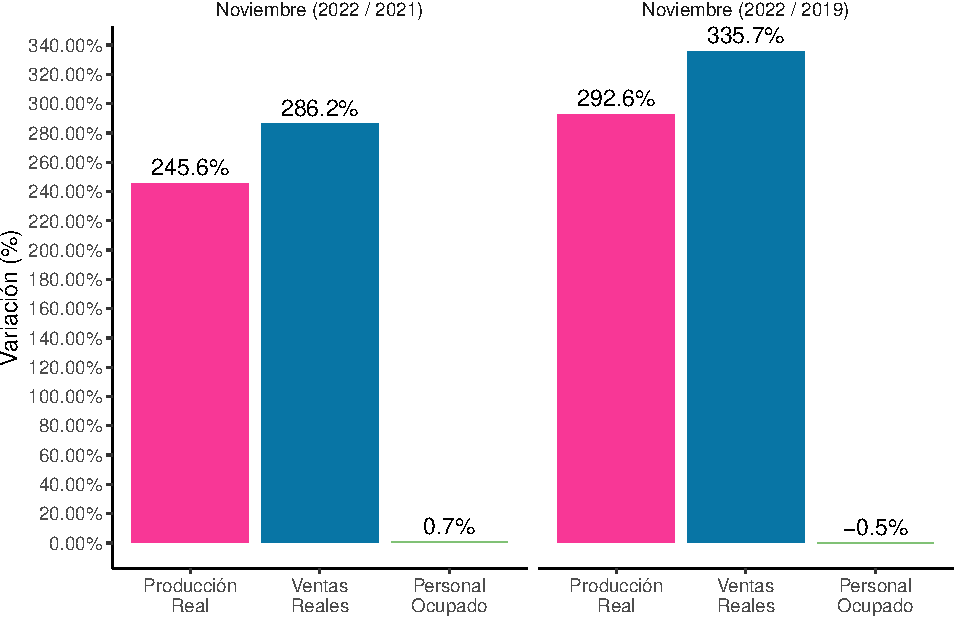
\includegraphics{boletin_files/figure-latex/variacion-1.pdf}

\textbf{Fuente}: DANE-EMMET\\
P: Cifras provisionales. Se presentan variaciones respecto al año 2020
para considerar el efecto base de comparación del periodo de pandemia.

\renewcommand\contentsname{}
\setcounter{tocdepth}{1}
\tableofcontents

\newpage

\hypertarget{introducciuxf3n}{%
\section*{Introducción}\label{introducciuxf3n}}

La Encuesta Mensual Manufacturera con Enfoque Territorial (EMMET), es
una investigación de carácter estadístico por medio de la cual el
Departamento Administrativo Nacional de Estadística (DANE) obtiene la
información de evolución de las principales variables económicas del
sector fabril colombiano en el corto plazo.

La EMMET mide la evolución mensual del sector manufactrero del país, a
través de las variables de producción, ventas, empleo, sueldos y horas
trabajadas; con ellas el DANE genera índice, variaciones y
contribuciones; es también una herramienta importante para la
elaboración de las estimaciones del Producto Interno Bruto (PIB) del
sector industrial que realiza la Dirección Técnica de Síntesis y Cuentas
Nacionales.

Tomando como marco la Encuesta Anual Manufacturera de 2017, se realizó
el último rediseño de la operación estadística. Sobre este año base, se
obtuvo una encuesta por muestreo no probabilístico de 3.100
establecimientos; con ellos se presentan los resultados a nivel total
nacional y su desagregación para 12 departamentos, Bogotá y otros
departamentos, 3 áreas metropolitanas y 8 ciudades del país, para los
diferentes usuarios públicos y privado. En el contexto nacional, se
mantienen 39 dominios industriales manufactureros de publicación
establecidos con base en la Clasificación Industrial Internacional
Uniforme (CIIU) de toas las actividades económicas Rev.~4 adaptada para
Colombia.De esta forma es posible obtener la información necesaria para
construir indicadores confiables de la industria manufacturera, los
cuales son herramientas importantes para la toma de decisiones
económicas en el país.

\hypertarget{evoluciuxf3n-general-de-las-principales-variables-total-nacional-noviembre-2022}{%
\section{Evolución general de las principales variables total nacional
Noviembre
2022}\label{evoluciuxf3n-general-de-las-principales-variables-total-nacional-noviembre-2022}}

En Noviembre de 2022 frente a Noviembre de 2021, la producción real de
la industria manufacturera presentó una variación de 245.6\%, las ventas
reales de de 286.2\% y el personal ocupado de 0.7\%.\\
\strut \\
\textbf{Gráfico 2. Variación anual de la producción real, ventas y personas ocupado de la industria manufacturera}\\
\textbf{Total Nacional}\\
\textbf{Enero 2020 – Noviembre 2022p}\\

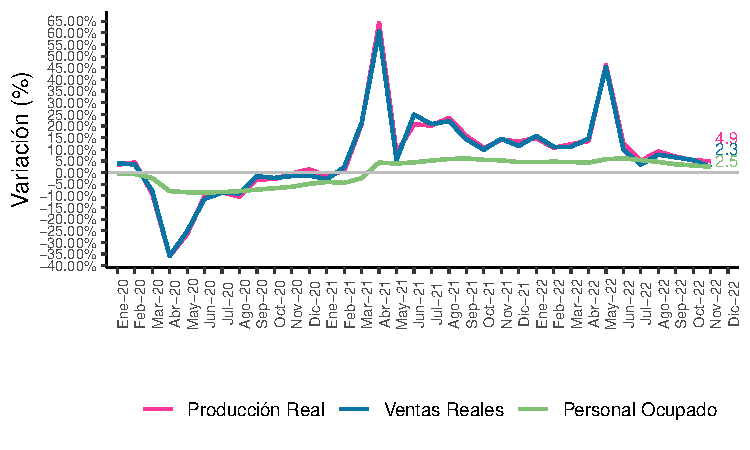
\includegraphics{boletin_files/figure-latex/historico-1.pdf}
\textbf{Fuente:} DANE- EMMET\\
P: Cifras provisionales\\

\hypertarget{variaciuxf3n-anual-y-contribuciuxf3n-del-valor-de-la-producciuxf3n-ventas-y-empleo-total-seguxfan-clase-industrial}{%
\subsection{Variación anual (\%) y contribución, del valor de la
producción, ventas y empleo total, según clase
industrial}\label{variaciuxf3n-anual-y-contribuciuxf3n-del-valor-de-la-producciuxf3n-ventas-y-empleo-total-seguxfan-clase-industrial}}

\textbf{Noviembre 2022/2021p}\\

De las 39 actividades industriales representadas por la encuesta, un
total de 19 registraron variaciones positivas en su producción real,
sumando 249.6 puntos porcentuales a la variación total anual y 20
subsectores con variaciones negativas restaron en conjunto -4.1 puntos
porcentuales a la variación total (Tabla1).

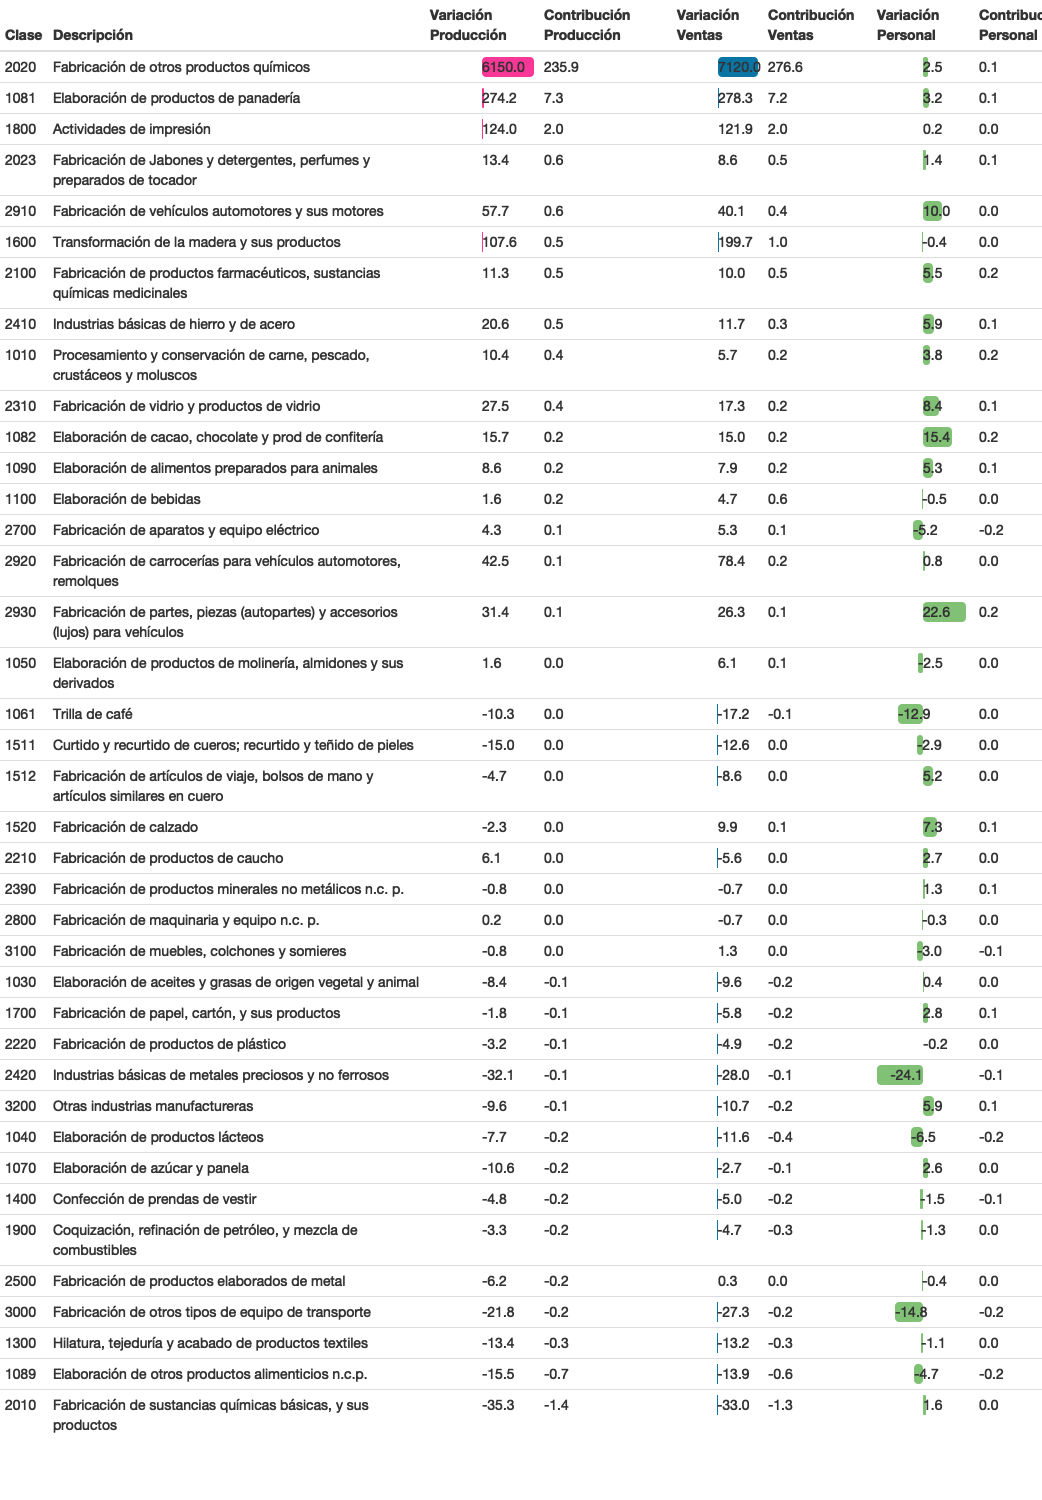
\includegraphics{boletin_files/figure-latex/tabla1_view-1.png}

\textbf{Fuente:} DANE- EMMET\\
P: Cifras provisionales\\
Nota: La diferencia en la suma se da por aproximaciones decimales\\
PP. Puntos porcentuales

\hypertarget{variaciuxf3n-auxf1o-corrido-y-contribuciuxf3n-del-valor-de-la-producciuxf3n-ventas-y-empleo-total-segpun-clase-industrial}{%
\subsection{Variación año corrido (\%) y contribución, del valor de la
producción, ventas y empleo total, segpun clase
industrial}\label{variaciuxf3n-auxf1o-corrido-y-contribuciuxf3n-del-valor-de-la-producciuxf3n-ventas-y-empleo-total-segpun-clase-industrial}}

\textbf{Enero - Noviembre 2022/2021p}\\
\strut \\

En lo corrido del año hastaNoviembre de 2022, la producción real de la
industria manufacturera presentó una variación de 36.1\%, las ventas
reales de 40.4\% y el personal ocupado de 4.3\%.\\

\textbf{Gráfico 3. Variación año corrido de la producción real, ventas y
personal ocupado de la industria manufacturera}\\
\textbf{Total nacional}\\
\textbf{Enero - 2020Noviembre 2022p}\\

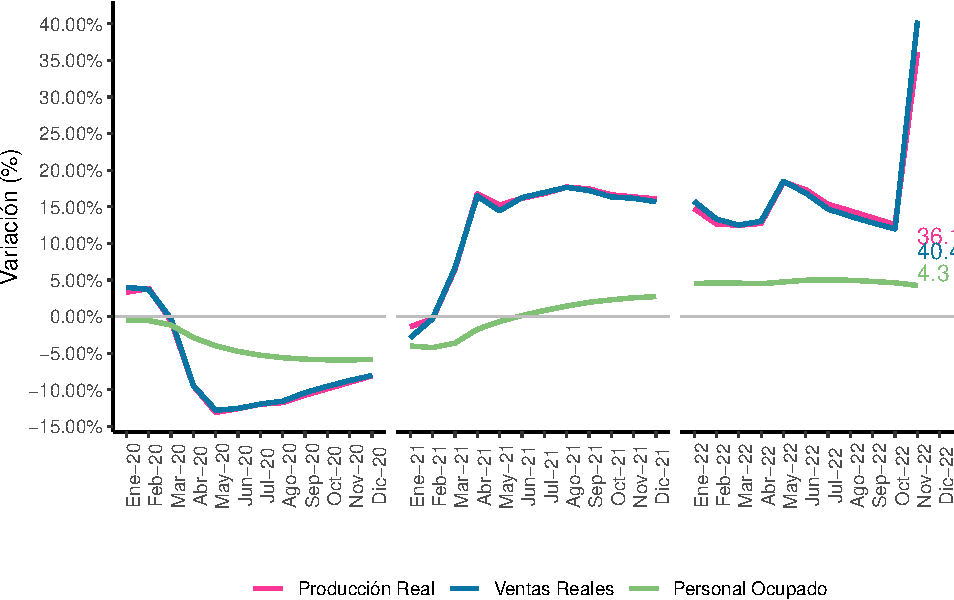
\includegraphics{boletin_files/figure-latex/anio_corrido_view-1.pdf}

\textbf{Fuente}: DANE-EMMET\\
P:Cifras provisionales\\

De las 39 actividades industriales representadas por la encuesta, un
total de 34 registraron variaciones positivas en su producción real,
sumando 36.5 puntos porcentuales a la variación total anual y 5
subsectores con variaciones negativas restaron en conjunto -0.1 puntos
porcentuales a la variación total (Tabla2).

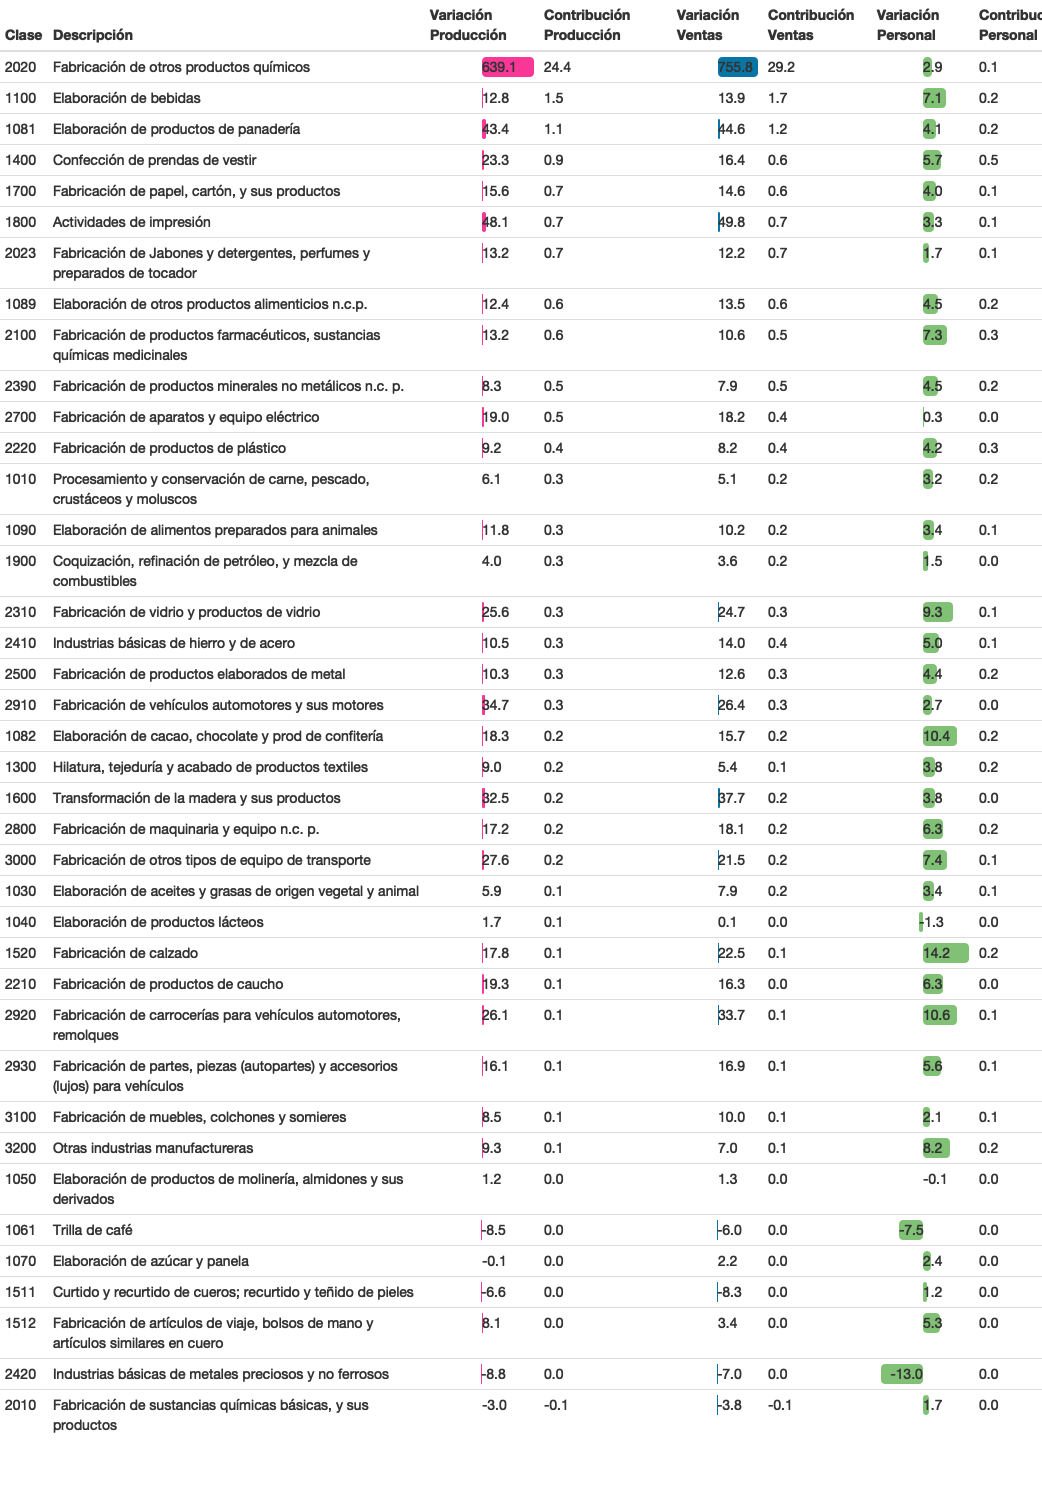
\includegraphics{boletin_files/figure-latex/tabla2_view-1.png}

\textbf{Fuente:} DANE-EMMET\\
P:Cifras provisionales\\
Nota: La diferencia en la suma se da por aproximaciones decimales\\
PP. Puntos porcentuales\\

\hypertarget{variaciuxf3n-doce-meses-y-contribuciuxf3n-del-valor-de-la-producciuxf3n-ventas-y-empleo-total-seguxfan-clase-industrial}{%
\subsection{1.3 Variación doce meses (\%) y contribución, del valor de
la producción, ventas y empleo total según clase
industrial}\label{variaciuxf3n-doce-meses-y-contribuciuxf3n-del-valor-de-la-producciuxf3n-ventas-y-empleo-total-seguxfan-clase-industrial}}

\textbf{Diciembre 2021 - Noviembre 2022 / Diciembre 2020 - Noviembre 2021P}\\
\textbf{Gráfico 4. Variación doce meses de la producción real, ventas y
personal ocupado de la industria manufacturera}\\
\textbf{Total nacional}\\
\textbf{Enero 2020 - Noviembre 2022P}\\

En lo corrido del año hastaNoviembre de 2022, la producción real de la
industria manufacturera presentó una variación de 34.2\%, las ventas
reales de 37.9\% y el personal ocupado de 4.3\%.\\

\textbf{Gráfico 3. Variación año corrido de la producción real, ventas y
personal ocupado de la industria manufacturera}\\
\textbf{Total nacional}\\
\textbf{Enero - 2020Noviembre 2022p}\\

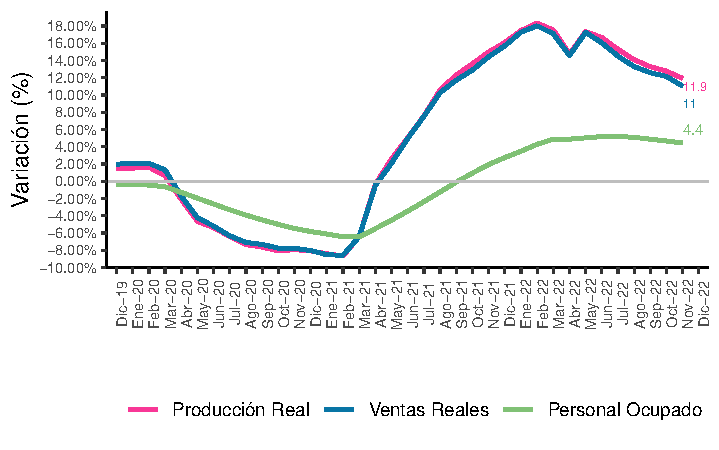
\includegraphics{boletin_files/figure-latex/anio_corrido_view_2-1.pdf}

\textbf{Fuente}: DANE-EMMET\\
P:Cifras provisionales\\

De las 39 actividades industriales representadas por la encuesta, un
total de 35 registraron variaciones positivas en su producción real,
sumando \ensuremath{1.125\times 10^{5}} puntos porcentuales a la
variación total doce meses y 4 subsectores con variaciones negativas
restaron en conjunto -2440 puntos porcentuales a la variación total.
(tabla 3)
\textbf{Tabla3. Variación doce meses y contribución de la producción real, ventas reales, y personal ocupado, según actividad manufacturera}\\
\textbf{Total Nacional}\\
\textbf{Diciembre 2021 - Noviembre 2022 / Diciembre 2020 - Noviembre 2021 P}

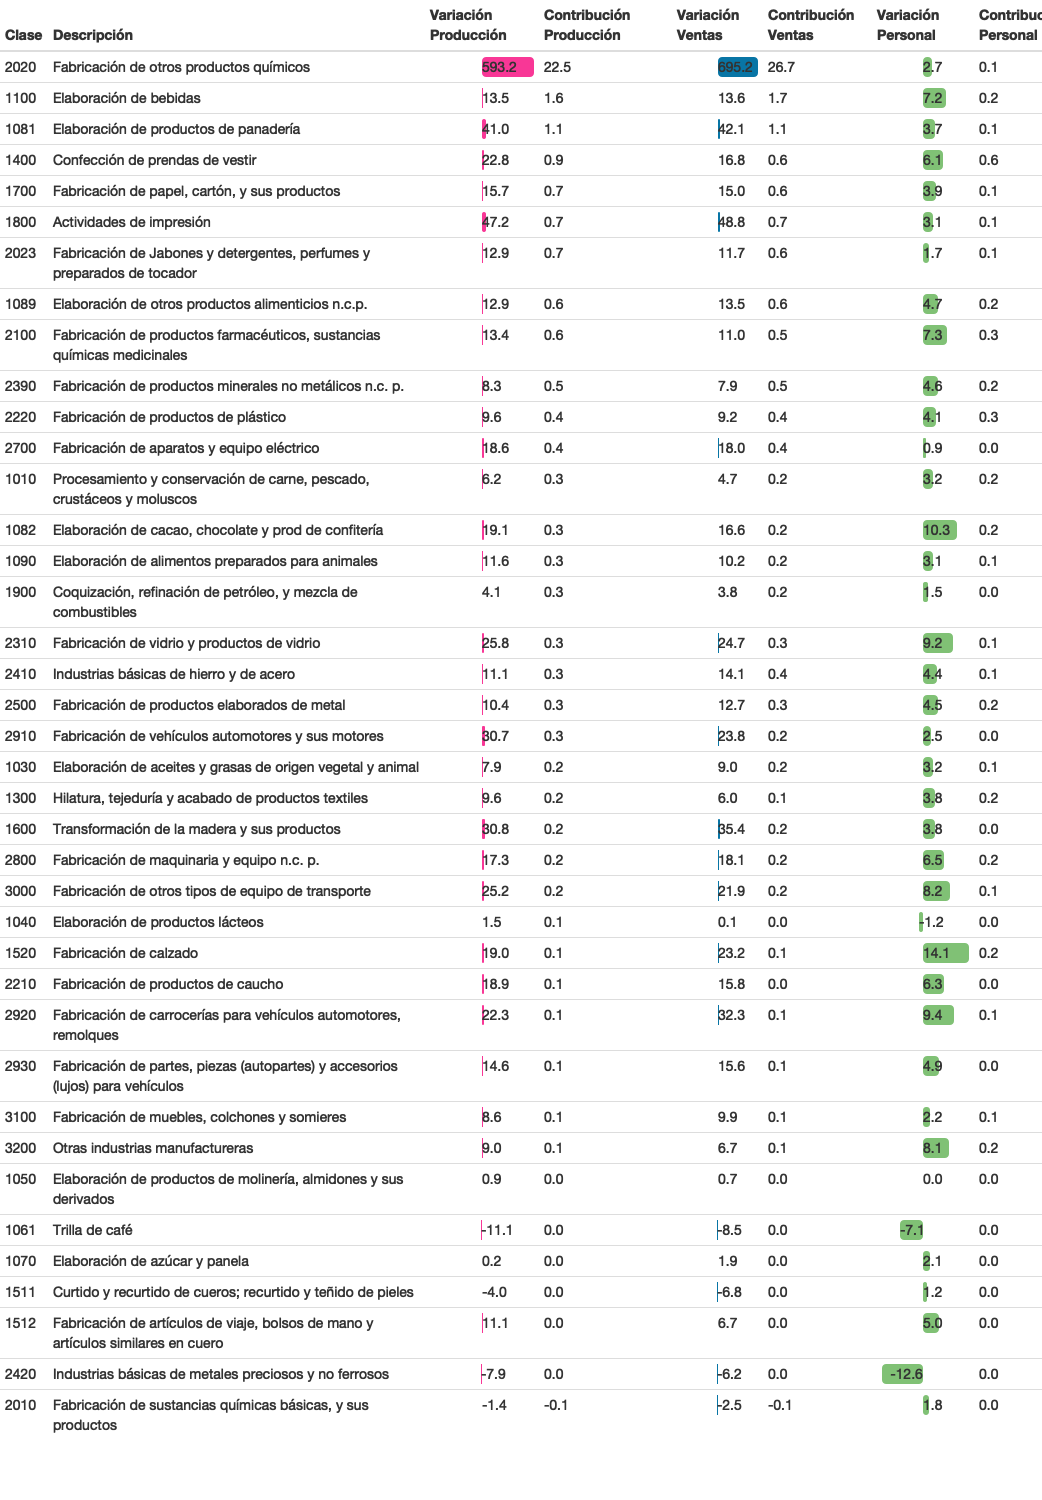
\includegraphics{boletin_files/figure-latex/tabla3_view-1.png}
\textbf{Fuente:} DANE-EMMET\\
P:Cifras provisionales\\
Nota: La diferencia en la suma se da por aproximaciones decimales\\
PP. Puntos porcentuales\\

\hypertarget{evoluciuxf3n-general-de-las-principales-variables-enfoque-territorial-noviembre-2022}{%
\section{Evolución general de las principales variables enfoque
territorial Noviembre
2022}\label{evoluciuxf3n-general-de-las-principales-variables-enfoque-territorial-noviembre-2022}}

\hypertarget{variaciuxf3n-anual-y-contribuciuxf3n-del-valor-de-la-producciuxf3n-ventas-y-empleo-total-seguxfan-departamentos}{%
\subsection{Variación anual (\%) y contribución, del valor de la
producción, ventas y empleo total según
departamentos}\label{variaciuxf3n-anual-y-contribuciuxf3n-del-valor-de-la-producciuxf3n-ventas-y-empleo-total-seguxfan-departamentos}}

De los 14 dominios de departamentos representado por la encuest,De los
14 dominios de departamentos representados por la encuesta, 10
registraron variaciones positivas en su producción real, sumando 3669.7
p.p. a la variación total nacional.\\
\strut \\
\textbf{Tabla 4. Variación anual y contribución de la producción real, ventas reales y personal ocupado}\\
\textbf{Departamentos} Noviembre (2022/2021)P
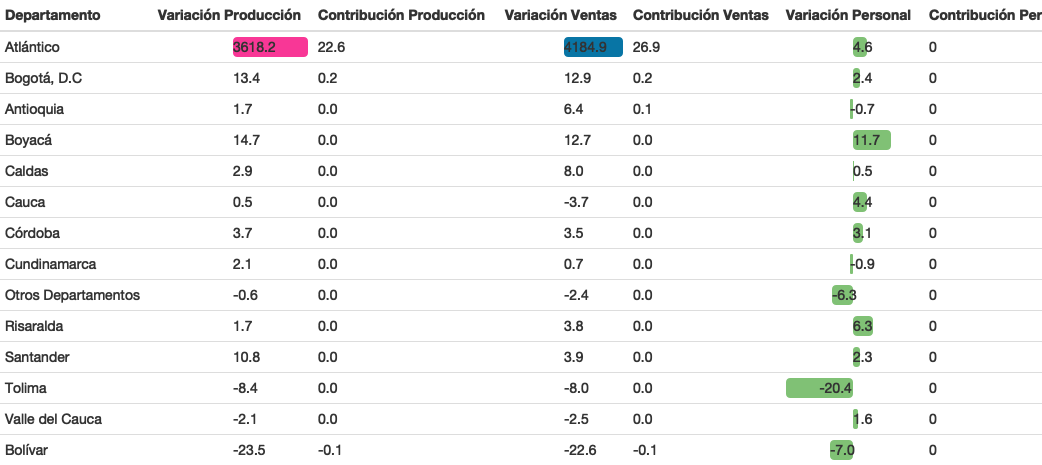
\includegraphics{boletin_files/figure-latex/tabla4_new-1.png}
\textbf{Fuente}: DANE-EMMET\\
P:Cifras provisionales\\
Nota: La diferencia en la suma se da por aproximaciones decimales\\
P.P. puntos porcentuales\\
* Otros departamentos: Amazonas, Caquetá, Casanare, Cesar, Chocó, Huila,
La Guajira, Magdalena, Meta, Nariño, Norte de Santander, Putumayo,
Quindío, San Andrés, Sucre.

\hypertarget{variaciuxf3n-anual-y-contribuciuxf3n-del-valor-de-la-producciuxf3n-ventas-y-empleo-total-seguxfan-uxe1reas-metropolitanas}{%
\subsection{Variación anual (\%) y contribución, del valor de la
producción, ventas y empleo total según áreas
metropolitanas}\label{variaciuxf3n-anual-y-contribuciuxf3n-del-valor-de-la-producciuxf3n-ventas-y-empleo-total-seguxfan-uxe1reas-metropolitanas}}

\textbf{Noviembre 2022/2021P}

En Noviembre de 2022 frente a Noviembre 2021, el área metropolitana que
más constribuye a la variación anual de la producción real es la de Área
Metropolitana de Barranquilla con una variación de
\ensuremath{3.6308\times 10^{5}}\%, sumando
\ensuremath{2.438\times 10^{4}} p.p. a la variación total nacional.\\
\strut \\

\textbf{Tabla 5. Variación anual y contribución de la producción real,
ventas reales y personal ocupado en Áreas Metropolitanas}\\
Noviembre (2022/2021)P

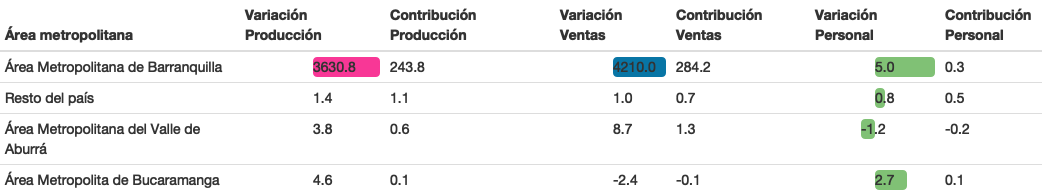
\includegraphics{boletin_files/figure-latex/tabl5_view-1.png}
\textbf{Fuente}: DANE-EMMET\\
P: Cifras provisionales\\
Nota: La diferencia en la suma se da por aproximaciones decimales\\
P.P. puntos porcentuales\\

\hypertarget{variaciuxf3n-anual-y-contribuciuxf3n-del-valor-de-la-producciuxf3n-ventas-y-empleo-total-seguxfan-ciudades}{%
\subsection{Variación anual (\%) y contribución, del valor de la
producción, ventas, y empleo total según
ciudades}\label{variaciuxf3n-anual-y-contribuciuxf3n-del-valor-de-la-producciuxf3n-ventas-y-empleo-total-seguxfan-ciudades}}

\textbf{Noviembre 2022/2021)P}\\
\strut \\

En Noviembre de 2022 frente a Noviembre de 2021 de los 10 dominios de
ciudades representados por la encuesta, 8 registraron variaciones
positivas en su producción real, sumando
\ensuremath{4.7185\times 10^{5}} p.p. de la variación total nacional
(tabla 6)\\
\strut \\
\textbf{Tabla 6. Variación anual y contribución de la producción real,
ventas reales y personal ocupado Ciudades}\\
\textbf{Noviembre 2022/2021)P}\\

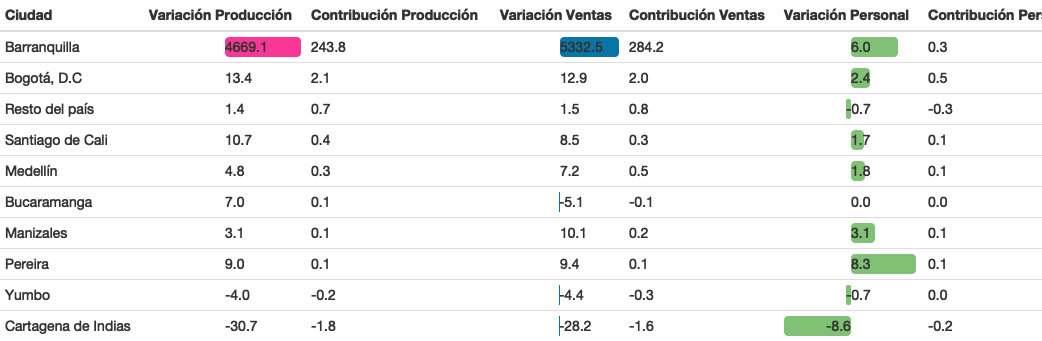
\includegraphics{boletin_files/figure-latex/tabla6_view-1.png}
\textbf{Fuente}: DANE-EMMET\\
P:Cifras provisionales\\
Nota: La diferencia en la suma se da por aproximaciones decimales\\
P.P. Puntos porcentuales\\

\hypertarget{variaciuxf3n-auxf1o-corrido-y-contribuciuxf3n-del-valor-de-la-producciuxf3n-ventas-y-empleo-total-seguxfan-departamentos}{%
\subsection{Variación año corrido (\%) y contribución, del valor de la
producción, ventas y empleo total, según
departamentos}\label{variaciuxf3n-auxf1o-corrido-y-contribuciuxf3n-del-valor-de-la-producciuxf3n-ventas-y-empleo-total-seguxfan-departamentos}}

\textbf{Enero - Noviembre 2022/2021P}\\
\strut \\

De los 14 dominio de departamentos representado por la encuesta,13
registraton variaciones positivas en su producción real, sumando
\ensuremath{5.071\times 10^{4}} p.p. a la variación total nacional
(Tabla 7)\\
\strut \\
\textbf{Tabla 7. Variación año corrido y contribución de la producción
real, ventas reales y personal ocupado}\\
\textbf{Departamentos}\\
\textbf{Enero - Noviembre 2022/2021P}\\

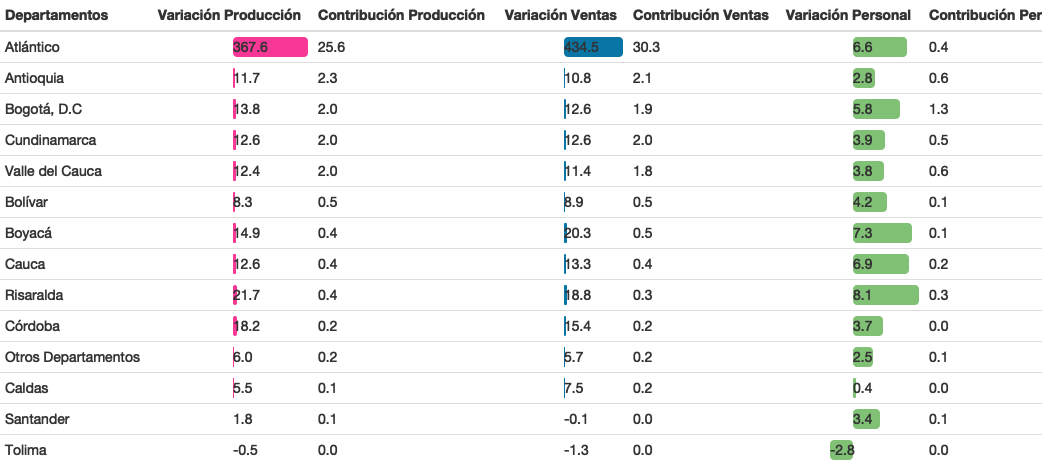
\includegraphics{boletin_files/figure-latex/tabla7_view-1.png}
\textbf{Fuente}: DANE-EMMET\\
P:Cifras provisionales\\
Nota: La diferencia en la suma se da por aproximaciones decimales\\
P.P. puntos porcentuales\\
* Otros departamentos: Amazonas, Caquetá, Casanare, Cesar, Chocó, Huila,
La Guajira, Magdalena, Meta, Nariño, Norte de Santander, Putumayo,
Quindío, San Andrés, Sucre.\\

\hypertarget{variaciuxf3n-auxf1o-corrido-y-contribuciuxf3n-del-valor-de-la-producciuxf3n-ventas-y-empleo-total-seguxfan-uxe1reas-metropolitanas}{%
\subsection{Variación año corrido (\%) y contribución, del valor de la
producción, ventas, y empleo total, según áreas
metropolitanas}\label{variaciuxf3n-auxf1o-corrido-y-contribuciuxf3n-del-valor-de-la-producciuxf3n-ventas-y-empleo-total-seguxfan-uxe1reas-metropolitanas}}

\textbf{Enero - Noviembre 2022/2021P}\\

En lo corrido del año hastaNoviembre de 2022, el área metropolitana que
más constribuye a la variación anual de la producción real es la de Área
Metropolitana de Barranquilla con una variación de
\ensuremath{3.697\times 10^{4}}\%, sumando 2550 p.p. a la variación
total nacional. (tabla 8)\\
\strut \\

\textbf{Tabla 8. Variación anual y contribución de la producción real,
ventas reales y personal ocupado}\\
\textbf{Áreas Metropolitanas}\\
Enero - Noviembre (2022/2021)P\\

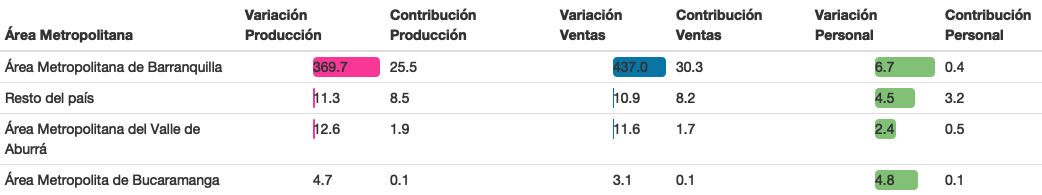
\includegraphics{boletin_files/figure-latex/tabla8_view-1.png}

\textbf{Fuente}: DANE-EMMET\\
P:Cifras provisionales\\
Nota: La diferencia en la suma se da por aproximaciones decimales\\
P.P. Puntos porcentuales\\

\hypertarget{variaciuxf3n-anual-y-contribuciuxf3n-del-valor-de-la-producciuxf3n-ventas-y-empleo-total-seguxfan-ciudades-1}{%
\subsection{Variación anual (\%) y contribución, del valor de la
producción, ventas, y empleo total según
ciudades}\label{variaciuxf3n-anual-y-contribuciuxf3n-del-valor-de-la-producciuxf3n-ventas-y-empleo-total-seguxfan-ciudades-1}}

\textbf{Enero - Noviembre 2022/2021)P}\\
\strut \\

En lo corrido del año hasta Noviembre de 2022, de los 10 dominios de
ciudades representados por la encuesta, 10 registraron variaciones
positivas en su producción real, sumando \ensuremath{5.739\times 10^{4}}
p.p. de la variación total nacional (tabla 9)\\
\strut \\
\textbf{Tabla 9. Variación anual y contribución de la producción real,
ventas reales y personal ocupado}\\
\textbf{Ciudades}\\
\textbf{Enero - Noviembre 2022/2021)P}\\

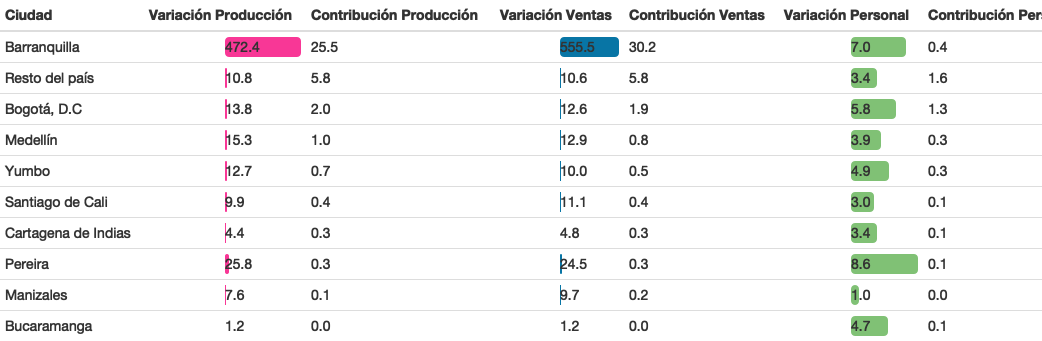
\includegraphics{boletin_files/figure-latex/tabla9_view-1.png}

\textbf{Fuente}: DANE-EMMET\\
P:Cifras provisionales\\
Nota: La diferencia en la suma se da por aproximaciones decimales\\
P.P. Puntos porcentuales\\

\hypertarget{variaciuxf3n-auxf1o-corrido-y-contribuciuxf3n-del-valor-de-la-producciuxf3n-ventas-y-empleo-total-seguxfan-departamentos-1}{%
\subsection{Variación año corrido (\%) y contribución, del valor de la
producción, ventas y empleo total, según
departamentos}\label{variaciuxf3n-auxf1o-corrido-y-contribuciuxf3n-del-valor-de-la-producciuxf3n-ventas-y-empleo-total-seguxfan-departamentos-1}}

\textbf{Diciembre 2021 - Noviembre 2022/Diciembre 2020 - Noviembre
2021P}\\
\strut \\

De los 14 dominios de departamentos representado por la encuesta,13
registraton variaciones positivas en su producción real, sumando
\ensuremath{4.816\times 10^{4}} p.p. a la variación total nacional
(Tabla 10)\\
\strut \\
\textbf{Tabla 10. Variación año corrido y contribución de la producción
real, ventas reales y personal ocupado}\\
\textbf{Departamentos}\\
\textbf{Diciembre 2021 - Noviembre 2022/Diciembre 2020 - Noviembre
2021P}\\

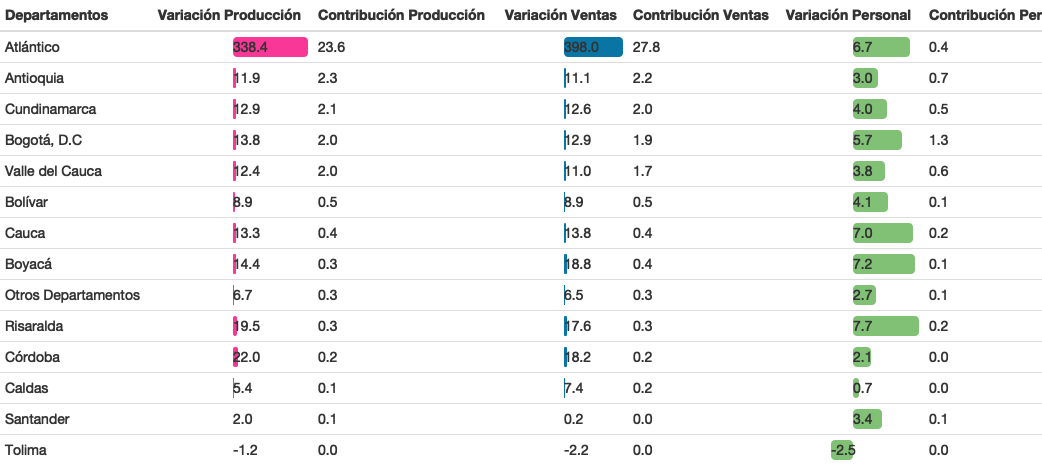
\includegraphics{boletin_files/figure-latex/tabla10_view-1.png}

\textbf{Fuente}: DANE-EMMET\\
P:Cifras provisionales\\
Nota: La diferencia en la suma se da por aproximaciones decimales\\
P.P. puntos porcentuales\\
* Otros departamentos: Amazonas, Caquetá, Casanare, Cesar, Chocó, Huila,
La Guajira, Magdalena, Meta, Nariño, Norte de Santander, Putumayo,
Quindío, San Andrés, Sucre.\\

\hypertarget{variaciuxf3n-auxf1o-corrido-y-contribuciuxf3n-del-valor-de-la-producciuxf3n-ventas-y-empleo-total-seguxfan-uxe1reas-metropolitanas-1}{%
\subsection{Variación año corrido (\%) y contribución, del valor de la
producción, ventas, y empleo total, según áreas
metropolitanas}\label{variaciuxf3n-auxf1o-corrido-y-contribuciuxf3n-del-valor-de-la-producciuxf3n-ventas-y-empleo-total-seguxfan-uxe1reas-metropolitanas-1}}

\textbf{Diciembre 2021 - Noviembre 2022/Diciembre 2020 - Noviembre
2021P}\\

Durante los últimos doce meses hasta el mes de Noviembre de 2022, el
área metropolitana que más constribuye a la variación anual de la
producción real es la de Área Metropolitana de Barranquilla con una
variación de \ensuremath{3.402\times 10^{4}}\%, sumando 2350 p.p. a la
variación total nacional. (tabla 11)\\
\strut \\

\textbf{Tabla 11. Variación anual y contribución de la producción real,
ventas reales y personal ocupado}\\
\textbf{Áreas Metropolitanas}\\
\textbf{Diciembre 2021 - Noviembre 2022/Diciembre 2020 - Noviembre
2021P}\\

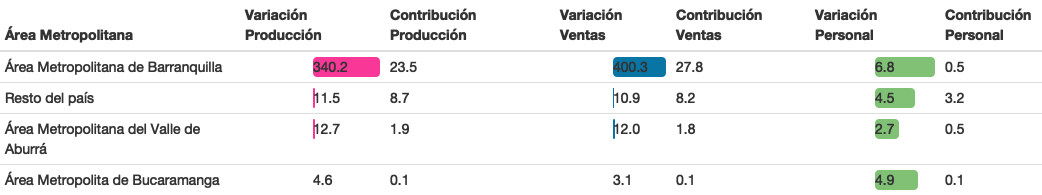
\includegraphics{boletin_files/figure-latex/tabla11_view-1.png}

\textbf{Fuente}: DANE-EMMET\\
P:Cifras provisionales\\
Nota: La diferencia en la suma se da por aproximaciones decimales\\
P.P. Puntos porcentuales\\

\hypertarget{variaciuxf3n-anual-y-contribuciuxf3n-del-valor-de-la-producciuxf3n-ventas-y-empleo-total-seguxfan-ciudades-2}{%
\subsection{Variación anual (\%) y contribución, del valor de la
producción, ventas, y empleo total según
ciudades}\label{variaciuxf3n-anual-y-contribuciuxf3n-del-valor-de-la-producciuxf3n-ventas-y-empleo-total-seguxfan-ciudades-2}}

\textbf{Diciembre 2021 - Noviembre 2022/Diciembre 2020 - Noviembre
2021P}\\

\hfill\break

Durante los últimos doce meses hasta Noviembre de 2022, de los 10
dominios de ciudades representados por la encuesta, 10 registraron
variaciones positivas en su producción real, sumando
\ensuremath{5.358\times 10^{4}} p.p. de la variación total nacional
(tabla 12)\\
\strut \\
\textbf{Tabla 12. Variación anual y contribución de la producción real,
ventas reales y personal ocupado}\\
\textbf{Ciudades}\\
\textbf{Diciembre 2021 - Noviembre 2022/Diciembre 2020 - Noviembre
2021P}\\

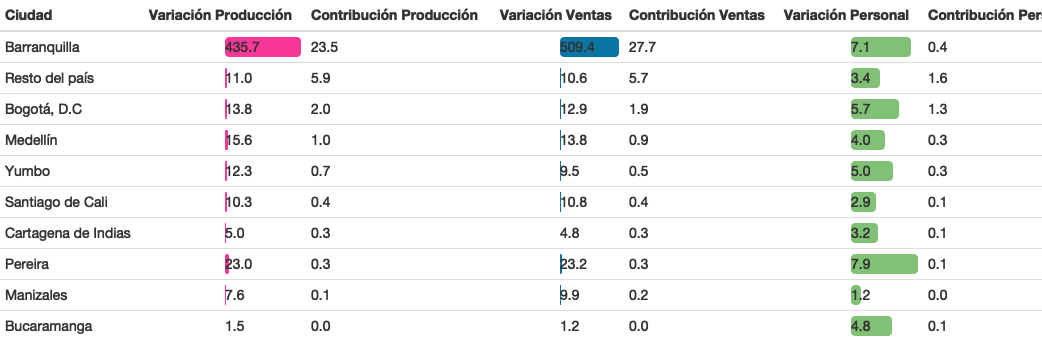
\includegraphics{boletin_files/figure-latex/tabla12_view-1.png}

\textbf{Fuente}: DANE-EMMET\\
P:Cifras provisionales\\
Nota: La diferencia en la suma se da por aproximaciones decimales\\
P.P. Puntos porcentuales\\

\hypertarget{evoluciuxf3n-general-de-las-principales-variables-total-nacional-variaciuxf3n-trienal-noviembre-2022}{%
\section{Evolución general de las principales variables total nacional
variación trienal Noviembre
2022}\label{evoluciuxf3n-general-de-las-principales-variables-total-nacional-variaciuxf3n-trienal-noviembre-2022}}

En Noviembre de 2022 frente al mismo mes de 2019, la producción real de
la industria manufacturera presentó una variación de frente al mismo mes
de 2019, la producción real de la industria manufacturera presentó una
variación de 245.6 \%, 292.6 \%, las ventas reales de 286.2 \%, 335.7 \%
y el personal ocupado 0.7 \%, -0.5 \%.\\
\strut \\
\textbf{Gráfico 5. Variación trienal de la producción real, ventas y
personal ocupado de la industria manufacturera}\\
\textbf{Total Nacional}\\
\textbf{Noviembre (2022/2021)P}\\

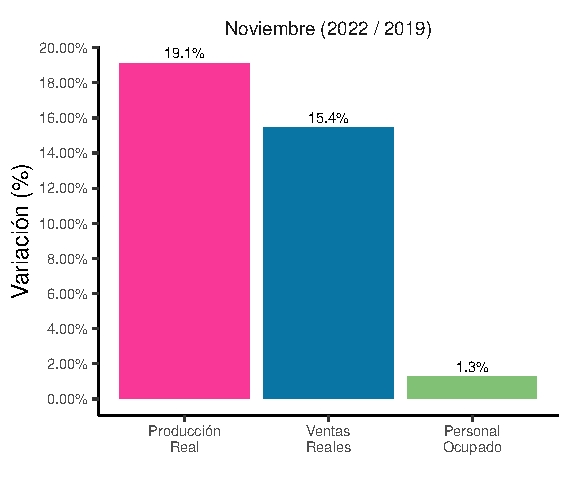
\includegraphics{boletin_files/figure-latex/variacion_trienal_plot-1.pdf}

\hypertarget{variaciuxf3n-trienal-y-contribuciuxf3n-del-valor-de-la-producciuxf3n-ventas-y-empleo-total-seguxfan-clase-industrial}{%
\subsection{Variación trienal (\%) y contribución, del valor de la
producción, ventas y empleo total según clase
industrial}\label{variaciuxf3n-trienal-y-contribuciuxf3n-del-valor-de-la-producciuxf3n-ventas-y-empleo-total-seguxfan-clase-industrial}}

\textbf{Noviembre (2022/2019)P}\\
\strut \\
De las 39 actividades industriales representadas por la encuesta, un
total de 30 registraron variaciones positivas en su producción real,
sumando \ensuremath{8.3222\times 10^{5}} puntos porcentuales a la
variación trienal y 9 subsectores con variaciones negativas restaron en
conjunto -8510 puntos porcentuales a la variación total (tabla 13).\\
\textbf{Tabla 13. variación trienal y contribución de la producción
real, ventas reales y personal ocupado, según actividad manufacturera}\\
\textbf{Total nacional}\\
\textbf{Noviembre (2022/2019)P}\\

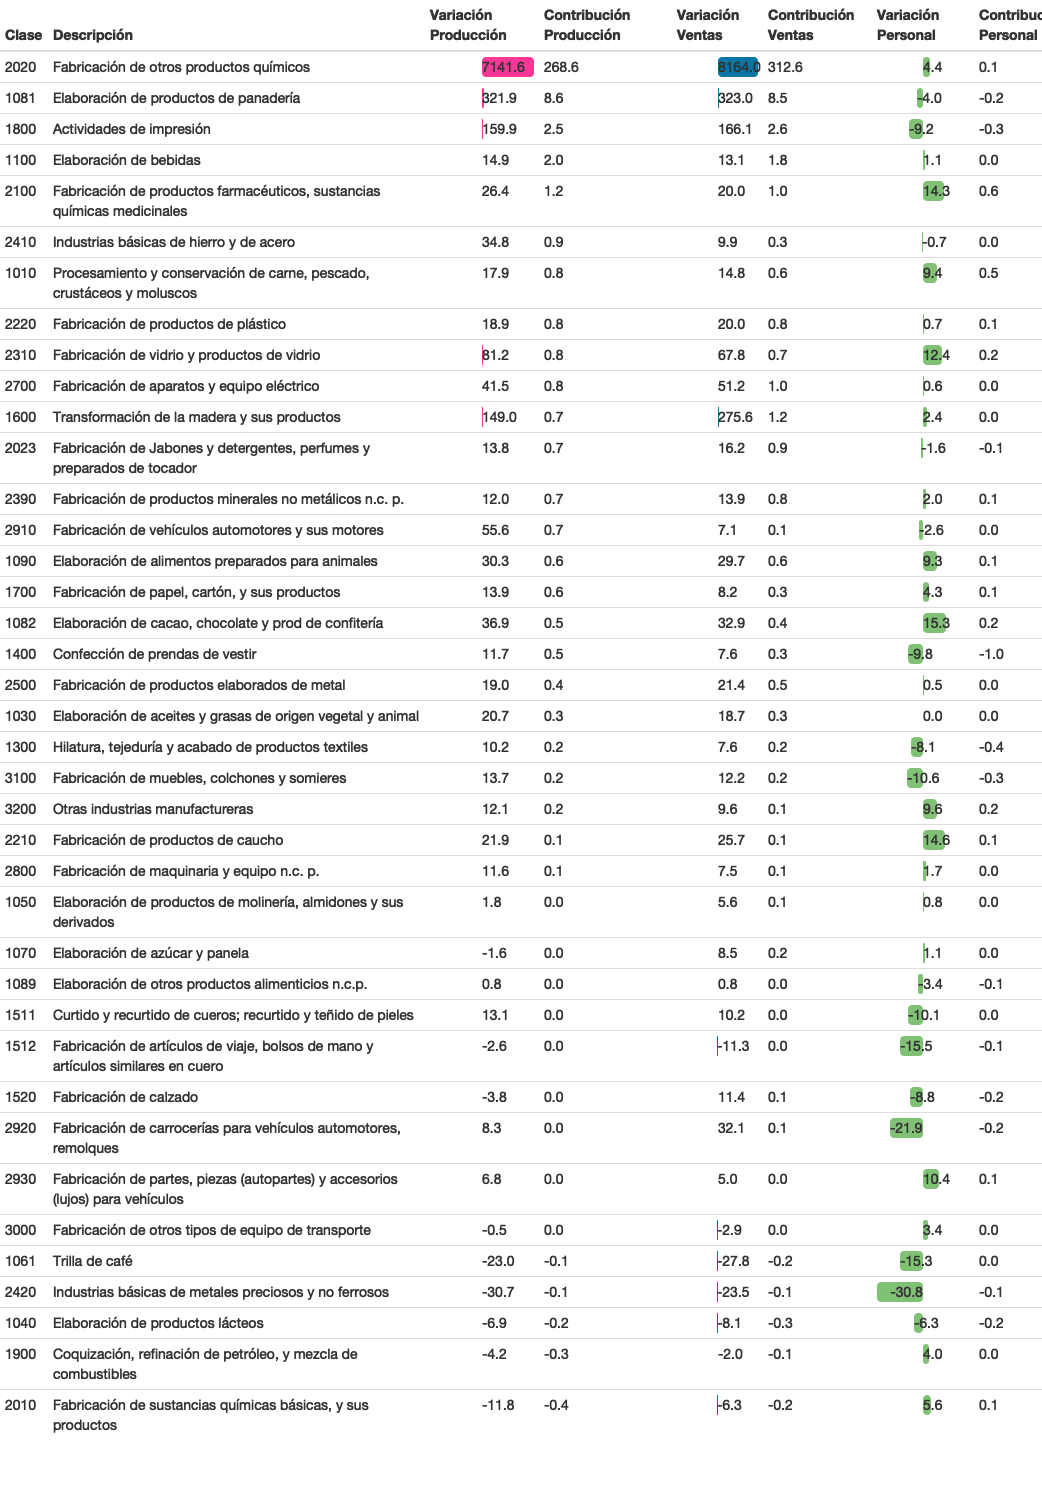
\includegraphics{boletin_files/figure-latex/tabla13_view-1.png}

\textbf{Fuente}: DANE-EMMET\\
P: Cifras provisionales\\
Nota: La diferencua en la suma se da por aproximaciones decimales\\
P.P. puntos porcentuales\\

\hypertarget{variaciuxf3n-trienal-y-contribuciuxf3n-del-valor-de-la-producciuxf3n-ventas-y-empleo-total-seguxfan-departamentos}{%
\subsection{Variación trienal (\%) y contribución, del valor de la
producción, ventas y empleo total según
departamentos}\label{variaciuxf3n-trienal-y-contribuciuxf3n-del-valor-de-la-producciuxf3n-ventas-y-empleo-total-seguxfan-departamentos}}

De los 14 dominios de departamentos representado por la encuest,De los
14 dominios de departamentos representados por la encuesta, 12
registraron variaciones positivas en su producción real, sumando 4435.3
p.p. a la variación total nacional.\\
\strut \\
\textbf{Tabla 4. Variación trienal y contribución de la producción real, ventas reales y personal ocupado}\\
\textbf{Departamentos} Noviembre (2022/2019)P\\

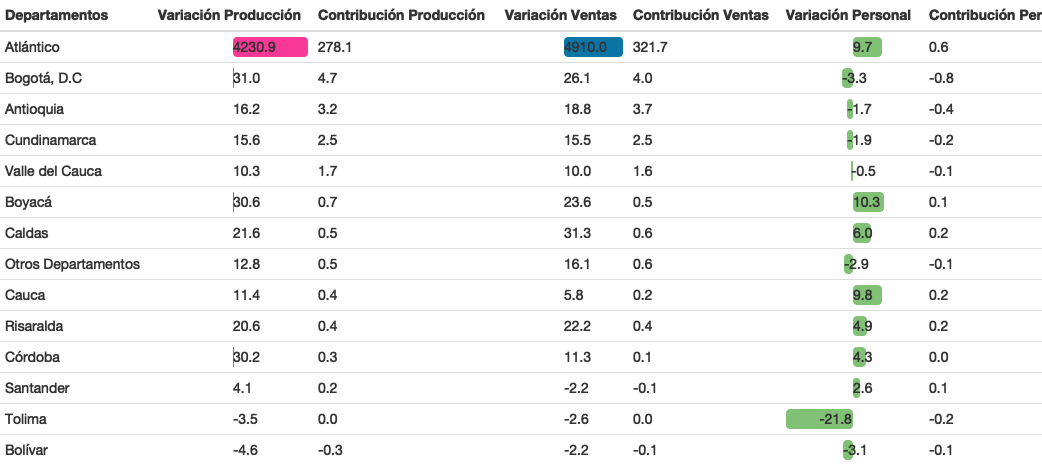
\includegraphics{boletin_files/figure-latex/tabla14_view-1.png}

\textbf{Fuente}: DANE-EMMET\\
P:Cifras provisionales\\
Nota: La diferencia en la suma se da por aproximaciones decimales\\
P.P. puntos porcentuales\\
* Otros departamentos: Amazonas, Caquetá, Casanare, Cesar, Chocó, Huila,
La Guajira, Magdalena, Meta, Nariño, Norte de Santander, Putumayo,
Quindío, San Andrés, Sucre.\\

\hypertarget{variaciuxf3n-trianual-y-contribuciuxf3n-del-valor-de-la-producciuxf3n-ventas-y-empleo-total-seguxfan-uxe1reas-metropolitanas}{%
\subsection{Variación trianual (\%) y contribución, del valor de la
producción, ventas y empleo total según áreas
metropolitanas}\label{variaciuxf3n-trianual-y-contribuciuxf3n-del-valor-de-la-producciuxf3n-ventas-y-empleo-total-seguxfan-uxe1reas-metropolitanas}}

\textbf{Noviembre 2022/2019P}\\

En Noviembre de 2022 frente al mismo mes del 2019, el área metropolitana
que más constribuye a la variación anual de la producción real es la de
Área Metropolitana de Barranquilla con una variación de
\ensuremath{4.2615\times 10^{5}}\%, sumando
\ensuremath{2.781\times 10^{4}} p.p. a la variación total nacional.
(Tabla 15)\\
\strut \\

\textbf{Tabla 15. Variación trienal y contribución de la producción
real, ventas reales y personal ocupado en Áreas Metropolitanas}\\
Noviembre (2022/2019)P\\

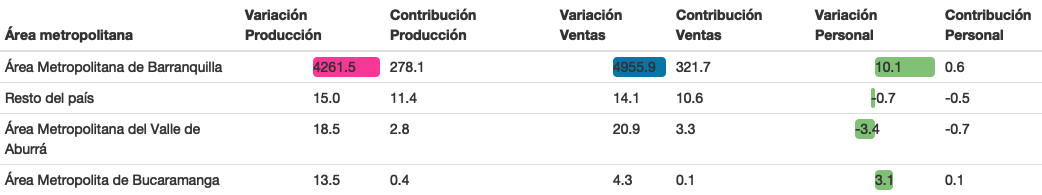
\includegraphics{boletin_files/figure-latex/tabla15_view-1.png}

\textbf{Fuente}: DANE-EMMET\\
P: Cifras provisionales\\
Nota: La diferencua en la suma se da por aproximaciones decimales\\
P.P. puntos porcentuales\\

\hypertarget{variaciuxf3n-trienal-y-contribuciuxf3n-del-valor-de-la-producciuxf3n-ventas-y-empleo-total-seguxfan-ciudades}{%
\subsection{Variación trienal (\%) y contribución, del valor de la
producción, ventas, y empleo total según
ciudades}\label{variaciuxf3n-trienal-y-contribuciuxf3n-del-valor-de-la-producciuxf3n-ventas-y-empleo-total-seguxfan-ciudades}}

\textbf{Noviembre 2022/2019)P}\\
\strut \\

En Noviembre de 2022 frente al mismo mes de 2019 de los 10 dominios de
ciudades representados por la encuesta, 9 registraron variaciones
positivas en su producción real, sumando
\ensuremath{5.7275\times 10^{5}} p.p. de la variación total nacional
(tabla 16)\\
\strut \\
\textbf{Tabla 16. Variación trienal y contribución de la producción
real, ventas reales y personal ocupado Ciudades}\\
\textbf{Noviembre 2022/2019)P}\\

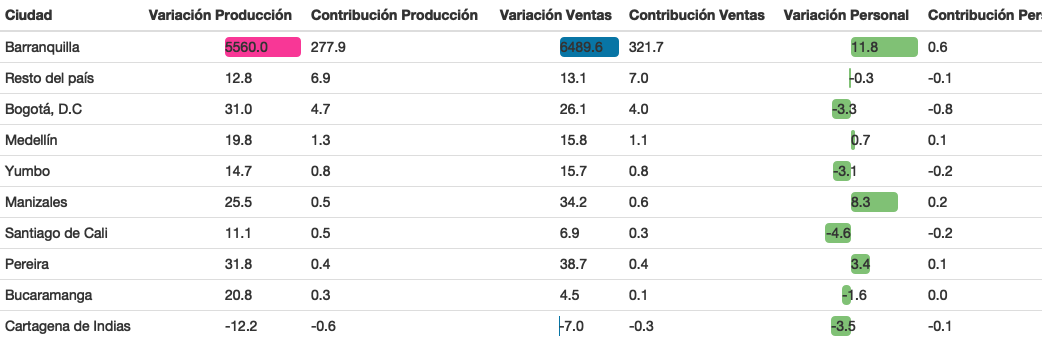
\includegraphics{boletin_files/figure-latex/tabla16_view-1.png}

\textbf{Fuente}: DANE-EMMET\\
P: Cifras provisionales\\
Nota: La diferencua en la suma se da por aproximaciones decimales\\
P.P. puntos porcentuales

\hypertarget{medidas-de-calidad}{%
\section{Medidas de calidad}\label{medidas-de-calidad}}

El porcentaje de cobertura es un instrumento que permite hacer
seguimiento al desarrollo de la recolección de infromación de los
establecimientos que hacen parte de la operación estadística.

Mide la relación entre la sumatoria del valor de las unidades
estadísticas de cobertura en la sumatoria del valor para total de las
unidades estadísticas de la muestra para las variables de diseño de la
operación. A mayor resultado, mayor cobertura de las variables de
importancia y diseño de la operación y mayor calidad de los resultados
publicados.

La fórmula para el cálculo del porcentaje de cobertura es:

\begin{equation*}
IC = \frac{(\sum H - \sum Hnc)}{\sum H}*100
\end{equation*} Donde, \(\sum H\), es la sumatoria del valor de la
variable \(H\) del total de las unidades estadpisticas de la
muestra.\textbackslash{} \(\sum Hnc\), es la sumatoria del valor de la
variable \(H\) de las unidades estadísticas de No Cobertura\}

\begin{align*}
ICProducción &= 98,1\%\\
ICVentas &= 98,1\%\\
ICEmpleo &= 98,5\%
\end{align*}

Para el caso de las unidades estadísticas que carecen de infromación por
presentar deuda en el periodo de estudio, se aplica el método de
imputación señalado en la metodología de la operación estadística.

\hypertarget{tasa-de-no-respuesta}{%
\subsection{Tasa de no respuesta}\label{tasa-de-no-respuesta}}

En este indicador se obtiene un resultado de qué porcentaje de las
fuentes esperadas no respondieron el formulario. La diferencia con el
indicador anterior es que considerando que hay un desgaste de la muestra
a medida que pasa el tiempo, hay fuentes de las cuales no se espera
información (fueron liquidadas, cambiaron de sector, etc). A menor
resultado, mayor calidad en los resultados publicados.

\begin{equation*}
TNR = \frac{\sum unr}{\sum ue}*100
\end{equation*} Donde,

\(\sum unr\), es la sumatoria de unidades estadísticas que no
respondieron el formulario\textbackslash{} \(\sum ue\), es la sumatoria
de unidades estadísticas esperadas

\begin{equation*}
TNR = 2,0\%
\end{equation*}

\hypertarget{tasa-de-imputaciuxf3n}{%
\subsection{Tasa de imputación}\label{tasa-de-imputaciuxf3n}}

La tasa de imputación mide el porcentaje de unidades estadísticas
imputadas del total de las unidades de la muestra. Se imputan datos
cuando hay deudas de formulario completo o parcial o en caso de que la
información sea incosistente. A menor resultado mayor calidad de los
datos publicados.

\begin{equation*}
TI = \frac{\sum uix}{\sum ux}*100
\end{equation*} Donde,

\(\sum uix\), es la sumatoria de unidades estadísticas imputadas en la
variable \(x\)\textbackslash{} \(\sum ux\), es la sumatoria de unidades
estadísticas de la muestra en la variable \(x\)

\begin{align*}
TIProducción &= 2,6\%\\
TIPVentas &= 2,5\%\\
TIEmpleo &= 2,7\%
\end{align*}

\hypertarget{ficha-metodoluxf3gica}{%
\section{Ficha Metodológica}\label{ficha-metodoluxf3gica}}

\textbf{Tipo de operación estadística}: encuesta por muestreo no
probabílistico, específicamente un muestreo de corte.\\
\strut \\
\textbf{Objetivo:} medir la evolución mensual del sector manufacturero
colombiano en el corto plazo, a través de las variables de producción,
ventas y empleo para la población objetivo, a total nacional y por
departamentos, áreas metropolitanas y ciudades.\\
\strut \\
\textbf{Alcance temático}: para la EMMET, los indicadores estarán
representados de manera mensual a nivel nacional por 39 dominios o
agrupaciones de la CIIU Rev.~4, que corresponde a las actividades
económicas del sector industria y que de acuerdo con la CIIU Rev.~4
A.C., se identifican como industria manufacturera y cumplen con los
parámetros de inclusión de la Encuesta Anual Manufacturera (10 o más
personas ocupadas o un nivel de producción igual o superio al
determinado cada año como parámetro de inclusión de la EAM). A nivel
nacional, desagregación territorial a nivel de departamentos, áreas
metropolitanas y ciudades. La EMMET no estudia el comportamiento de las
microempresas, considerando que el sector manufacturero nacional tienen
una distribución asímetrica y los establecimientos con mayor nivel de
producción son los que más influyen en su comportamiento.\\
\strut \\
\textbf{Indicadores:} los datos acerca de las características de los
establecimientos industriales. manufactureros son recopilados con fines
estadísticos para agregarlos a nivel de dominios y total del sector. Con
esta información se obtiene el índice de producción industrial
manufacturera (IPIM), el cual permite conocer la estructura y evolución
del sector manufacturero en Colombia. Estándares estadísticos empleados:
+ Clasificación Industrial Internacional Uniforme - CIIU Revisión 4 A.C.
+ División Político Administrativa - Divipola + Clasificación Central de
Productos ver 2 - CPC 2.\\
\strut \\
\textbf{Unidades Estadísticas}: la unidad de observación, análisis y
muestro es el establecimiento industrial.\\
\strut \\
\textbf{Universo de estudio}: está constituido por los establecimientos,
que de acuerdo con la CIIU Rev.~4 A.C., se clasifican como industria
manufacturera, desarrollan sus actividades en el territorio nacional y
emplean diez (10) o más personas o superan un nivel determinado de
producción anualmente establecido en la EAM.\\
\strut \\
\textbf{Población objetivo}: los establecimiento industrailes
manufactureros en el país que ocupand diez (10) o más personas y que en
suma produjeron el 80\% de la producción industrial reportada por la EAM
2017 y concentran el 65\% del empleo total; en cada dominio de estudio
publicado (dominio para departamento, área metropolitana, ciudad).\\
\strut \\
\textbf{Tamaño de muestra}: el tamaño total de la EMMET, según este
diseño, fue de 3.100 establecimientos industriales manufactureros,
resultado de la muestra requerida para cumplir con los cortes en cada
uno de los dominios de estudio del orden nacional y territorial.
\textbf{Cobertura geográfica}: total nacional.\\
\strut \\
\textbf{Desagregación geográfica}: totales a nivel nacional, 12
departamentos, 3 áreas metropoliutanas, 8 ciudades.\\
\strut \\
\textbf{Desagregación temática}: 39 dominios industriales según CIIU
Rev.~4 y de acuerdo con la clasificación CIIU 4, se presentan 56
sub-dominios industriales según el cruce dominio departamento.\\
\strut \\
\textbf{Periodo de referencia}: la información hace referencia a dos
meses atrás al mes en que se difunde la información; es decir, si la
información se difunde en el mes de febrero la información hace
referencia a diciembre. Existe un rezago de 45 días entre la publicaciín
y el mes de referencia.\\
\strut \\
\textbf{Periodo y periodicidad de recolección}: la recolección de
infromación se realiza durante los 25 días siguientes al mes de
referencia y la periodicidad de recolección es mensual.\\
\strut \\
\textbf{Método de recolección y acopio}: formulario electrónico,
autodiligenciado con asesoría en las casos que se requiera.

\hypertarget{glosario}{%
\section{Glosario}\label{glosario}}

\textbf{Principales términos utilizados}:

\textbf{La industria manufacturera:} es quella que ``abarca la
transformación física o química de materiales, sustancias o componentes
en productos nuevos''. DANE, 2012, CIIU Rev.~4 A.C., pág. 111.\\

\textbf{Establecimiento}: ``Empresa o parate de una empresa que, de
manera independiente, se dedica exclusivamente a un tipo de actividad
económica en una emplazamiento o desde un emplazamiento o dentro de una
zona geográfica y respecto de la cual, como unidad estadística de
observación, existen o pueden recopilarse con alguna precisión de datos
que permitan calcular la producción y sus costos''. DANE, 2012, CIIU
Rev.~4 A.C.\\

\textbf{Empresa}: ``Entidad institucional en su calidad de productora de
bienes y servicios. Es un agente económico con autonomía para adoptar
decisiones financieras y de inversión y con autoridad y responsabilidad
para asignar recursos a la producción de bienes y servicios y que puede
realizar una o varias actividades productivas''. DANE, 2012, CIIU Rev.~4
A.C.\\

\textbf{Actividad económica}: ``Es la creación de valor agregado
mediante la producción de bienes y servicios en la que intervienen la
tierra, el capital, el trabajo y los insumos intermedios''. DANE, 2012,
CIIU Rev.~4 A.C.\\

\textbf{Personas ocupado}: ``Corresponde al personal que labora en la
empresa o establecimiento, contratado de forma directo por ésta o a
través de empresas especializadas, y a los propietarios, socios y
familiares sin remuneración fija''. DANE, 2012, CIIU Rev.~4 A.C.\\

\textbf{Producción nominal}: valor de los productos elaborados y los
subproductos y desechos que resultan de la producción y que se destinan
a la venta, valor de los productos manufacturados para terceros que
entregan la materia prima, valor de los ingresos por servicios
industriales, valorados a precio promdio de venta en fábrica y sin
incluir los impuestos indirectos (IVA, consumo, etc.).\\

\textbf{Producción real}: valor nominal de la producción deflactada por
el índice de precios al productos según clase industrial.\\

\textbf{Ventas nominales}: valor de los productos y subproductos
elaborados por el establecimiento y vendidos durante el mes de
referencia, a precio de venta en fábrica y sin incluir los impuestos
indirectos. Incluye también aquellos productos elaborados por otros
establecimientos a los cuales se haya suministrado la materia prima para
su transofmración, el valor cobrado por los productos elaborados por
terceros, industriales y no industriales y el valor de los ingresos por
servicios industriales préstados. El valor de ventas se precisa según
destino, así: ventas realizadas en el país y al exterior.\\

\textbf{Ventas reales}: valor nominal de las ventas deflactadas por el
índice de precios al productos según clase industrial.\\

\textbf{Horas trabajadas}: se define como el total de horas que el
personasl de produccción ha trabajado efectivamente durante el periodo
de información, es decir, al número de horas laboradas y no al número de
horas pagadas, razón por la cual se excluye el tiempo correspondiente a
permisos remunerados, vacaciones, ausencias por enfermedad, dominicales
y festivos no trabajados.\\

\textbf{Sueldos}: se entiende por sueldos y salarios la retribución fija
u ordinaria que el persona (permanente o contratado directamente por el
establecimiento) percibe como pago por los servicios prestados durante
el periodo al que se refiere la información, antes de deducir los
descuentos por retención en la fuente, seguro social, sindicatom fondo
de empleados y similaresm etc. Incluye salarios básicos, sobresueldos y
bonificaciones mensuales permanentes ( por mayor costo de vida,
condiciones ambientales, riesgos, etc.), pago a los trabajadores a
destajo o por producción, pagos por trabajos en horas extras o en días
de descanso obligatorio, recargos nocturnos y festivos, licencias por
enfermedad o maternidad pagadas directamente por el patrono, comisiones
o porcentajes sobre ventas y mayor producción, viáticos cuando son
permanentes.\\

También se cuenta con desagregación de personal y salarios según
funcionalidad (administrativo o producción) o según contratación
(permanente temporal). \newpage


\includegraphics[width=18cm]{img/infodane.png}

\end{document}
